\subsubsection{Análisis para $C_{comp_{3}}$ en modo corriente, $I_{out} = 2 \si[per-mode=symbol]{\ampere}$, $R_{L} = 0 \si[per-mode=symbol]{\ohm}$}
% CCOMP3 MODO 3.

\clearpage

\begin{figure}[H] %htb
\begin{center}
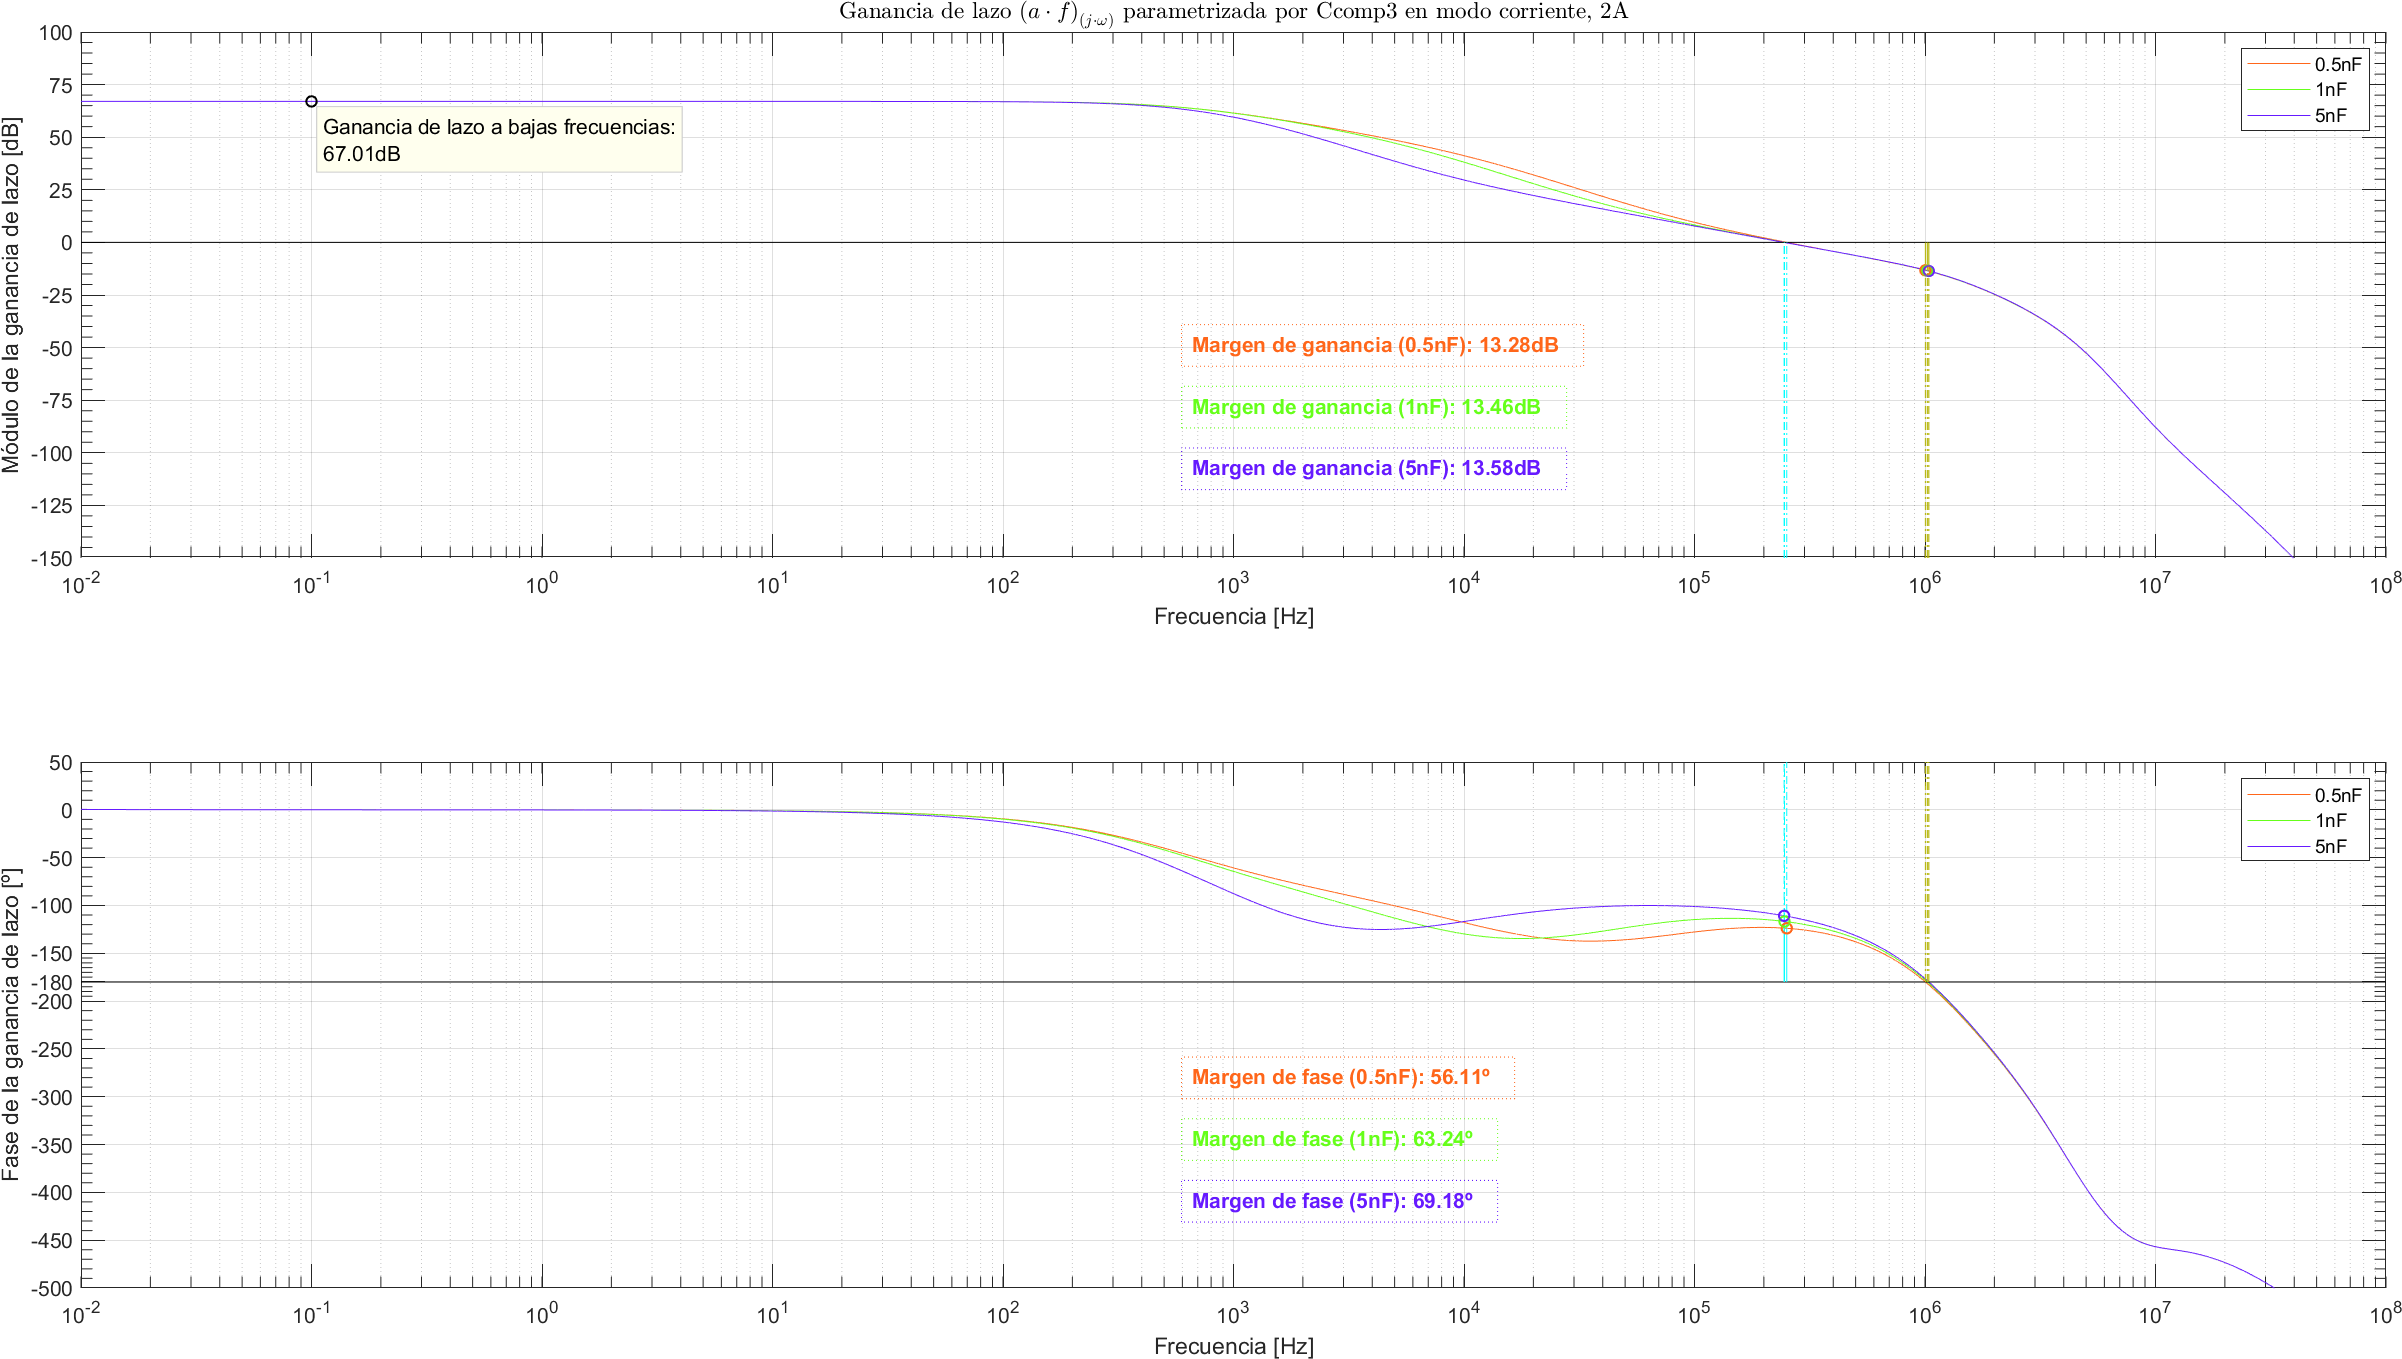
\includegraphics[width=1.1 \textwidth, angle=90]{./img/plots/loop/power_supply_CCOMP3_LOOP_Modo3.png}
\caption{\label{fig:fig_power_supply_CCOMP3_LOOP_Modo3}\footnotesize{Ganancia de lazo en modo corriente, $I_{out} = 2 \si[per-mode=symbol]{\ampere}$, en función de la frecuencia parametrizada por $C_{comp_{3}}$.}}
\end{center}
\end{figure}


\clearpage

\begin{figure}[H] %htb
\begin{center}
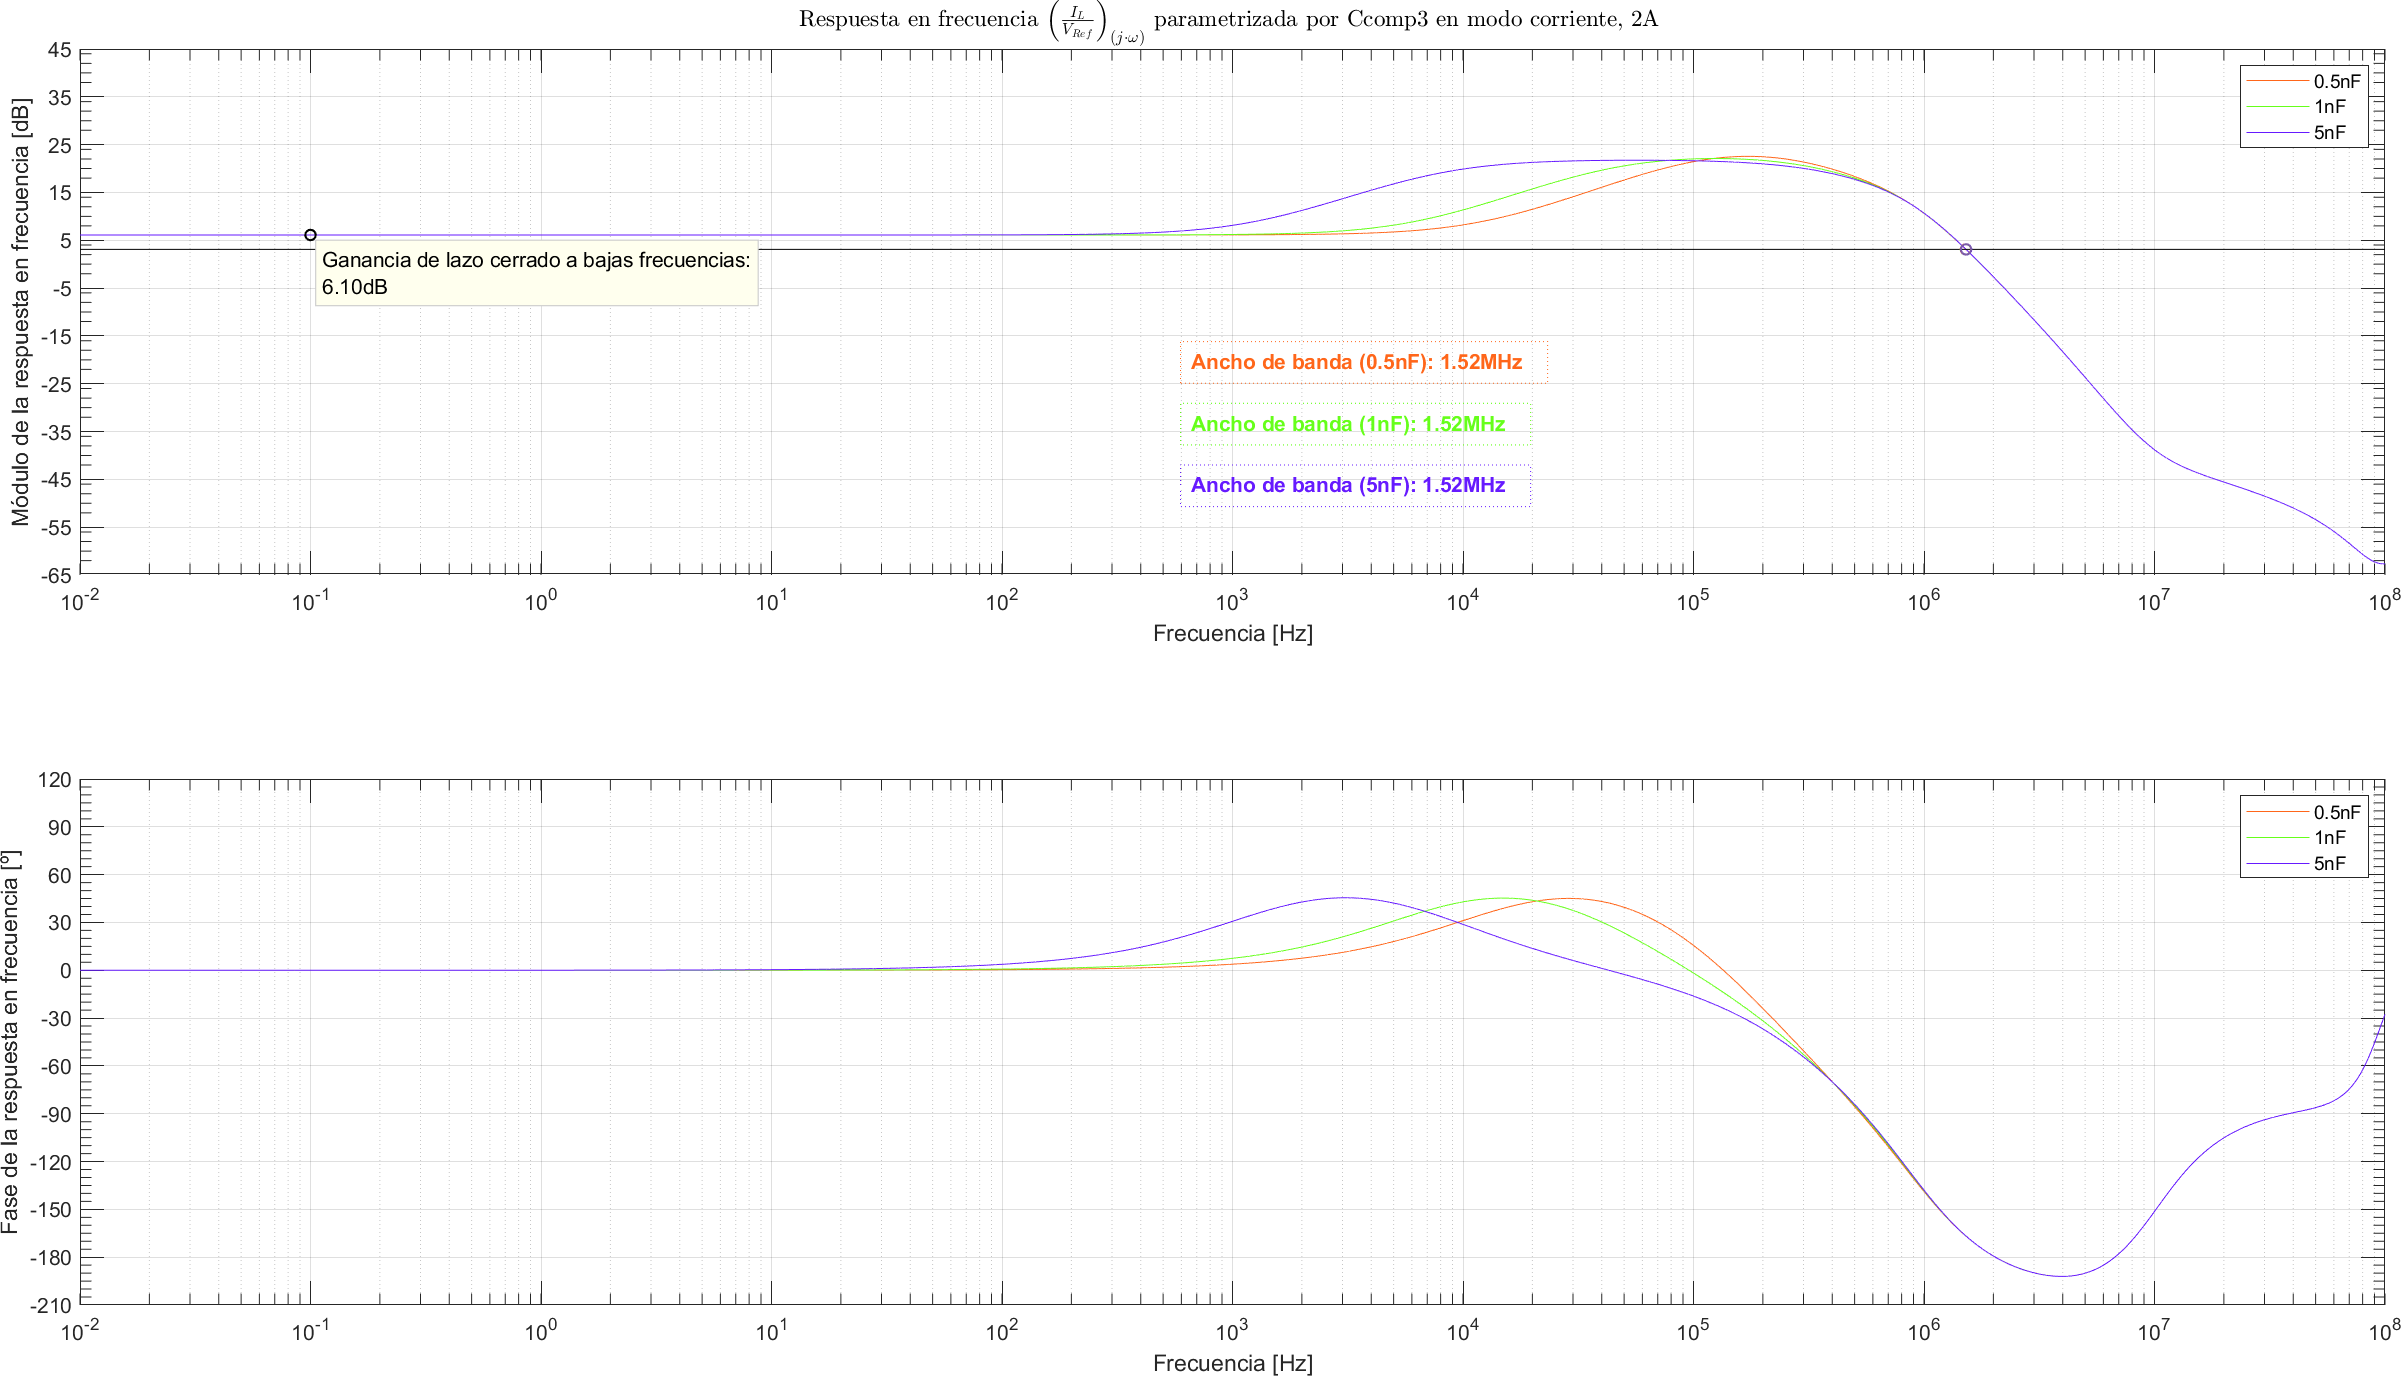
\includegraphics[width=1.1 \textwidth, angle=90]{./img/plots/rf/power_supply_CCOMP3_RF_Modo3.png}
\caption{\label{fig:fig_power_supply_CCOMP3_RF_Modo3}\footnotesize{Respuesta en frecuencia en modo corriente, $I_{out} = 2 \si[per-mode=symbol]{\ampere}$, en función de la frecuencia parametrizada por $C_{comp_{3}}$.}}
\end{center}
\end{figure}

\clearpage

\begin{figure}[H] %htb
\begin{center}
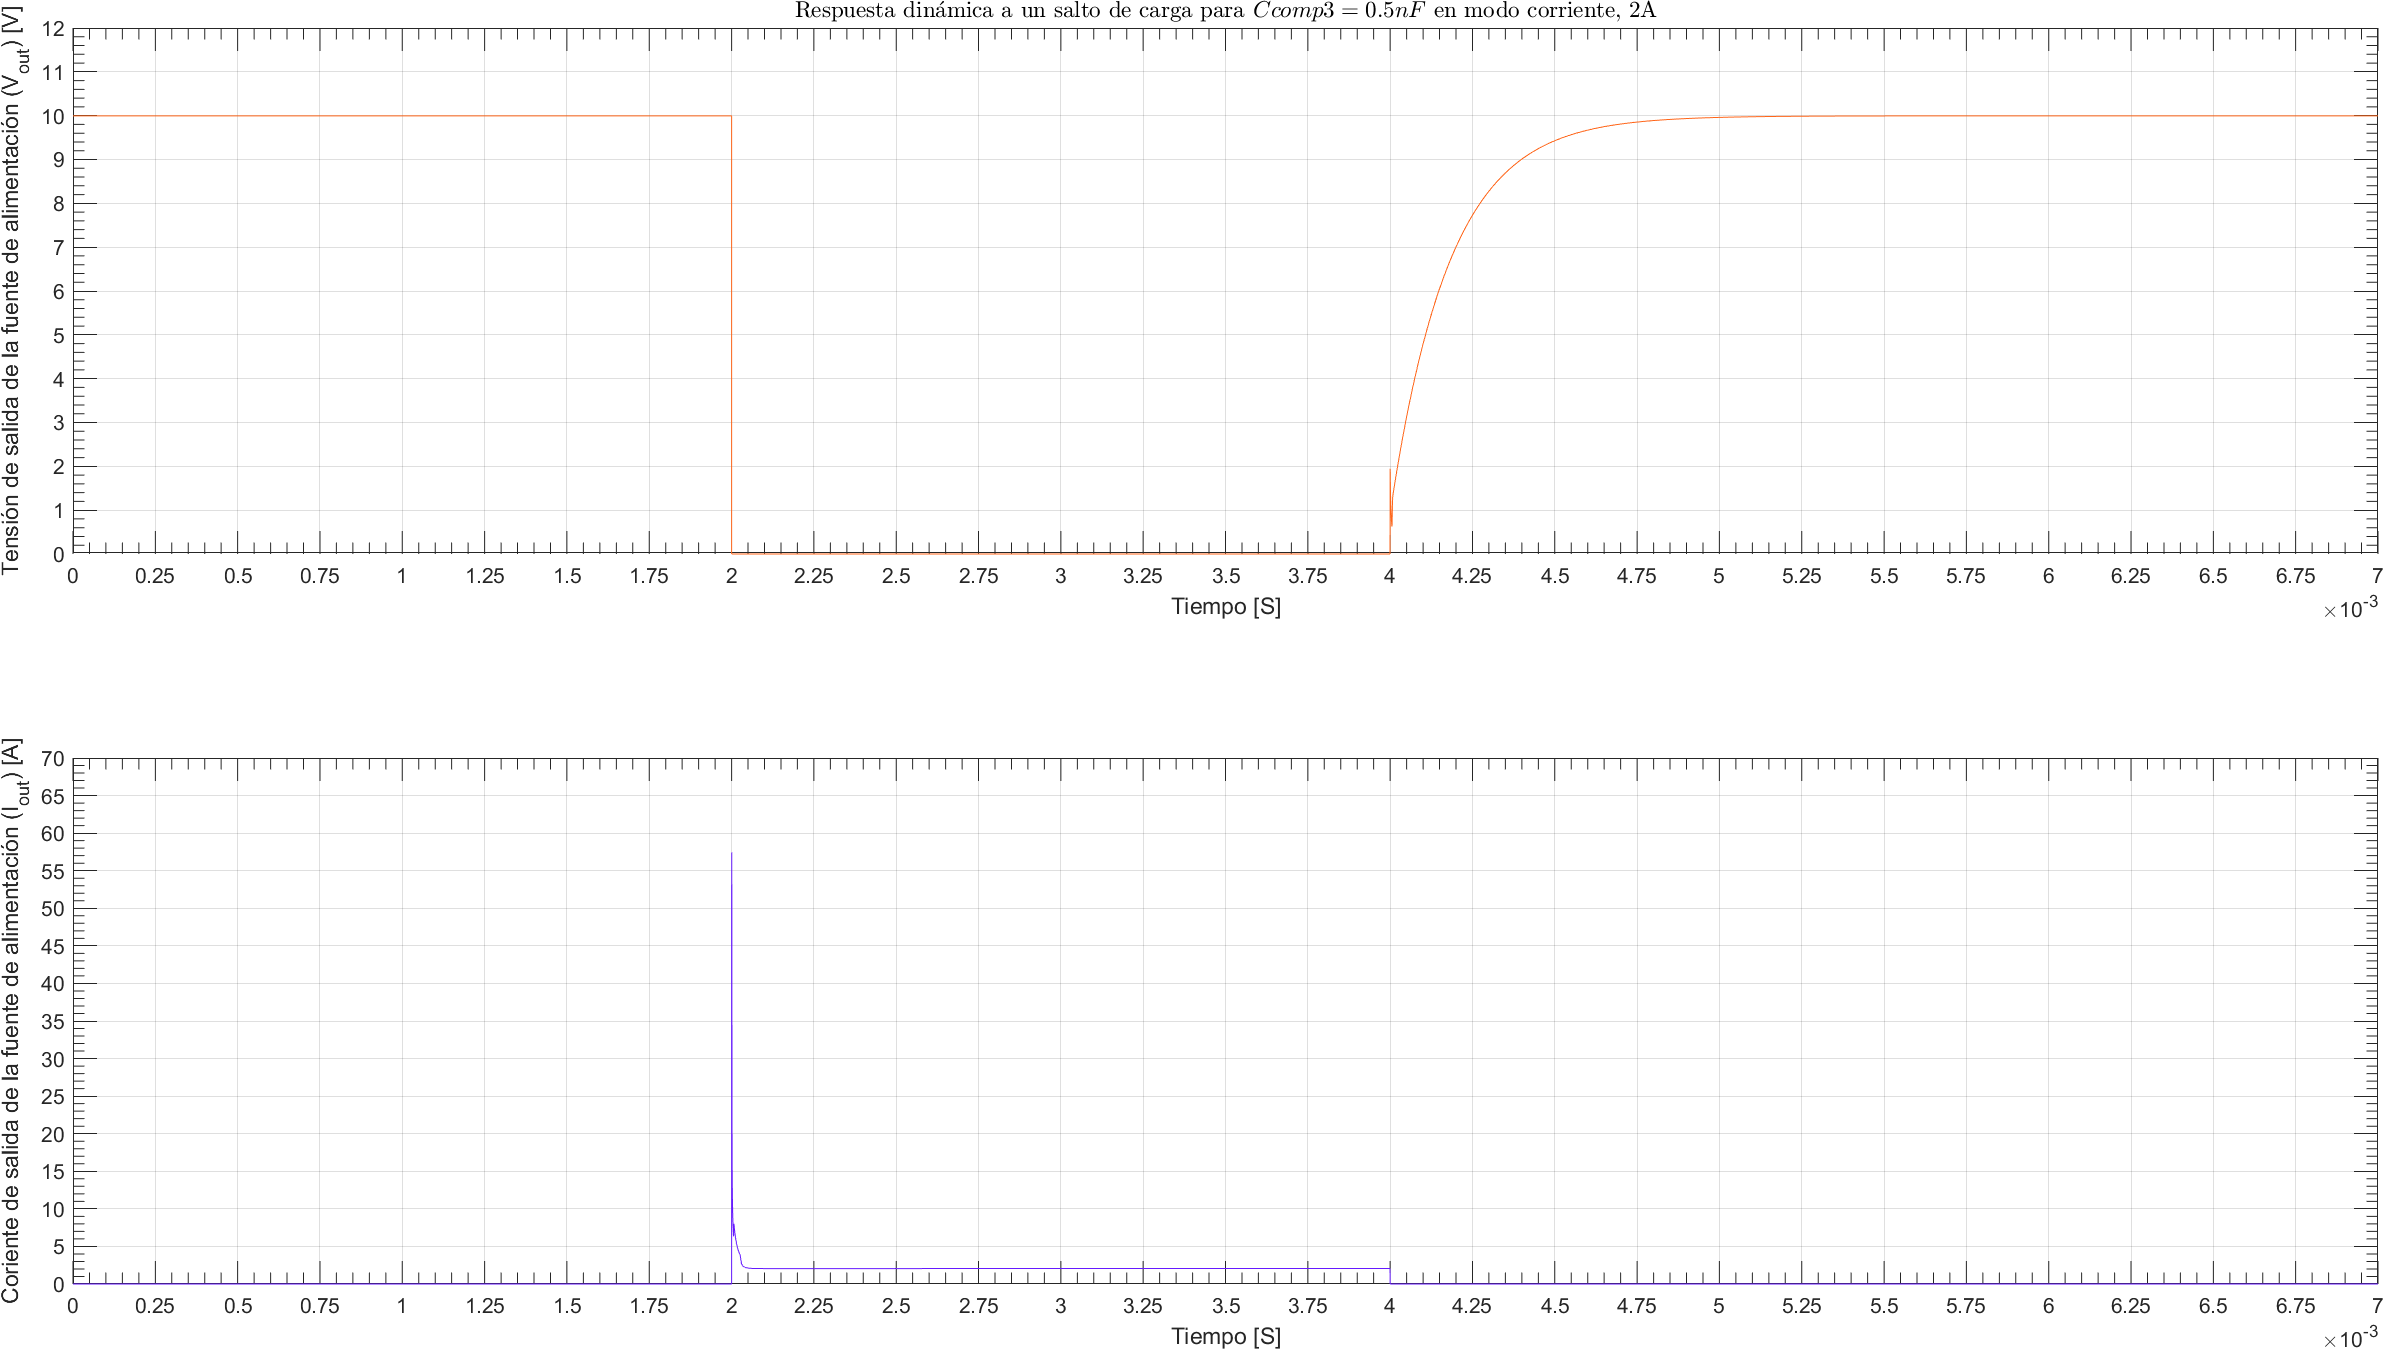
\includegraphics[width=1.1 \textwidth, angle=90]{./img/plots/dynamic/power_supply_CCOMP3_0_5n_STEP_Modo3.png}
\caption{\label{fig:fig_power_supply_CCOMP3_STEP_0_5n_Modo3}\footnotesize{Respuesta dinámica en modo corriente, $I_{out} = 2 \si[per-mode=symbol]{\ampere}$, para $C_{comp_{3}} = 0.5 \si[per-mode=symbol]{\nano\farad} $.}}
\end{center}
\end{figure}

\clearpage

\begin{figure}[H] %htb
\begin{center}
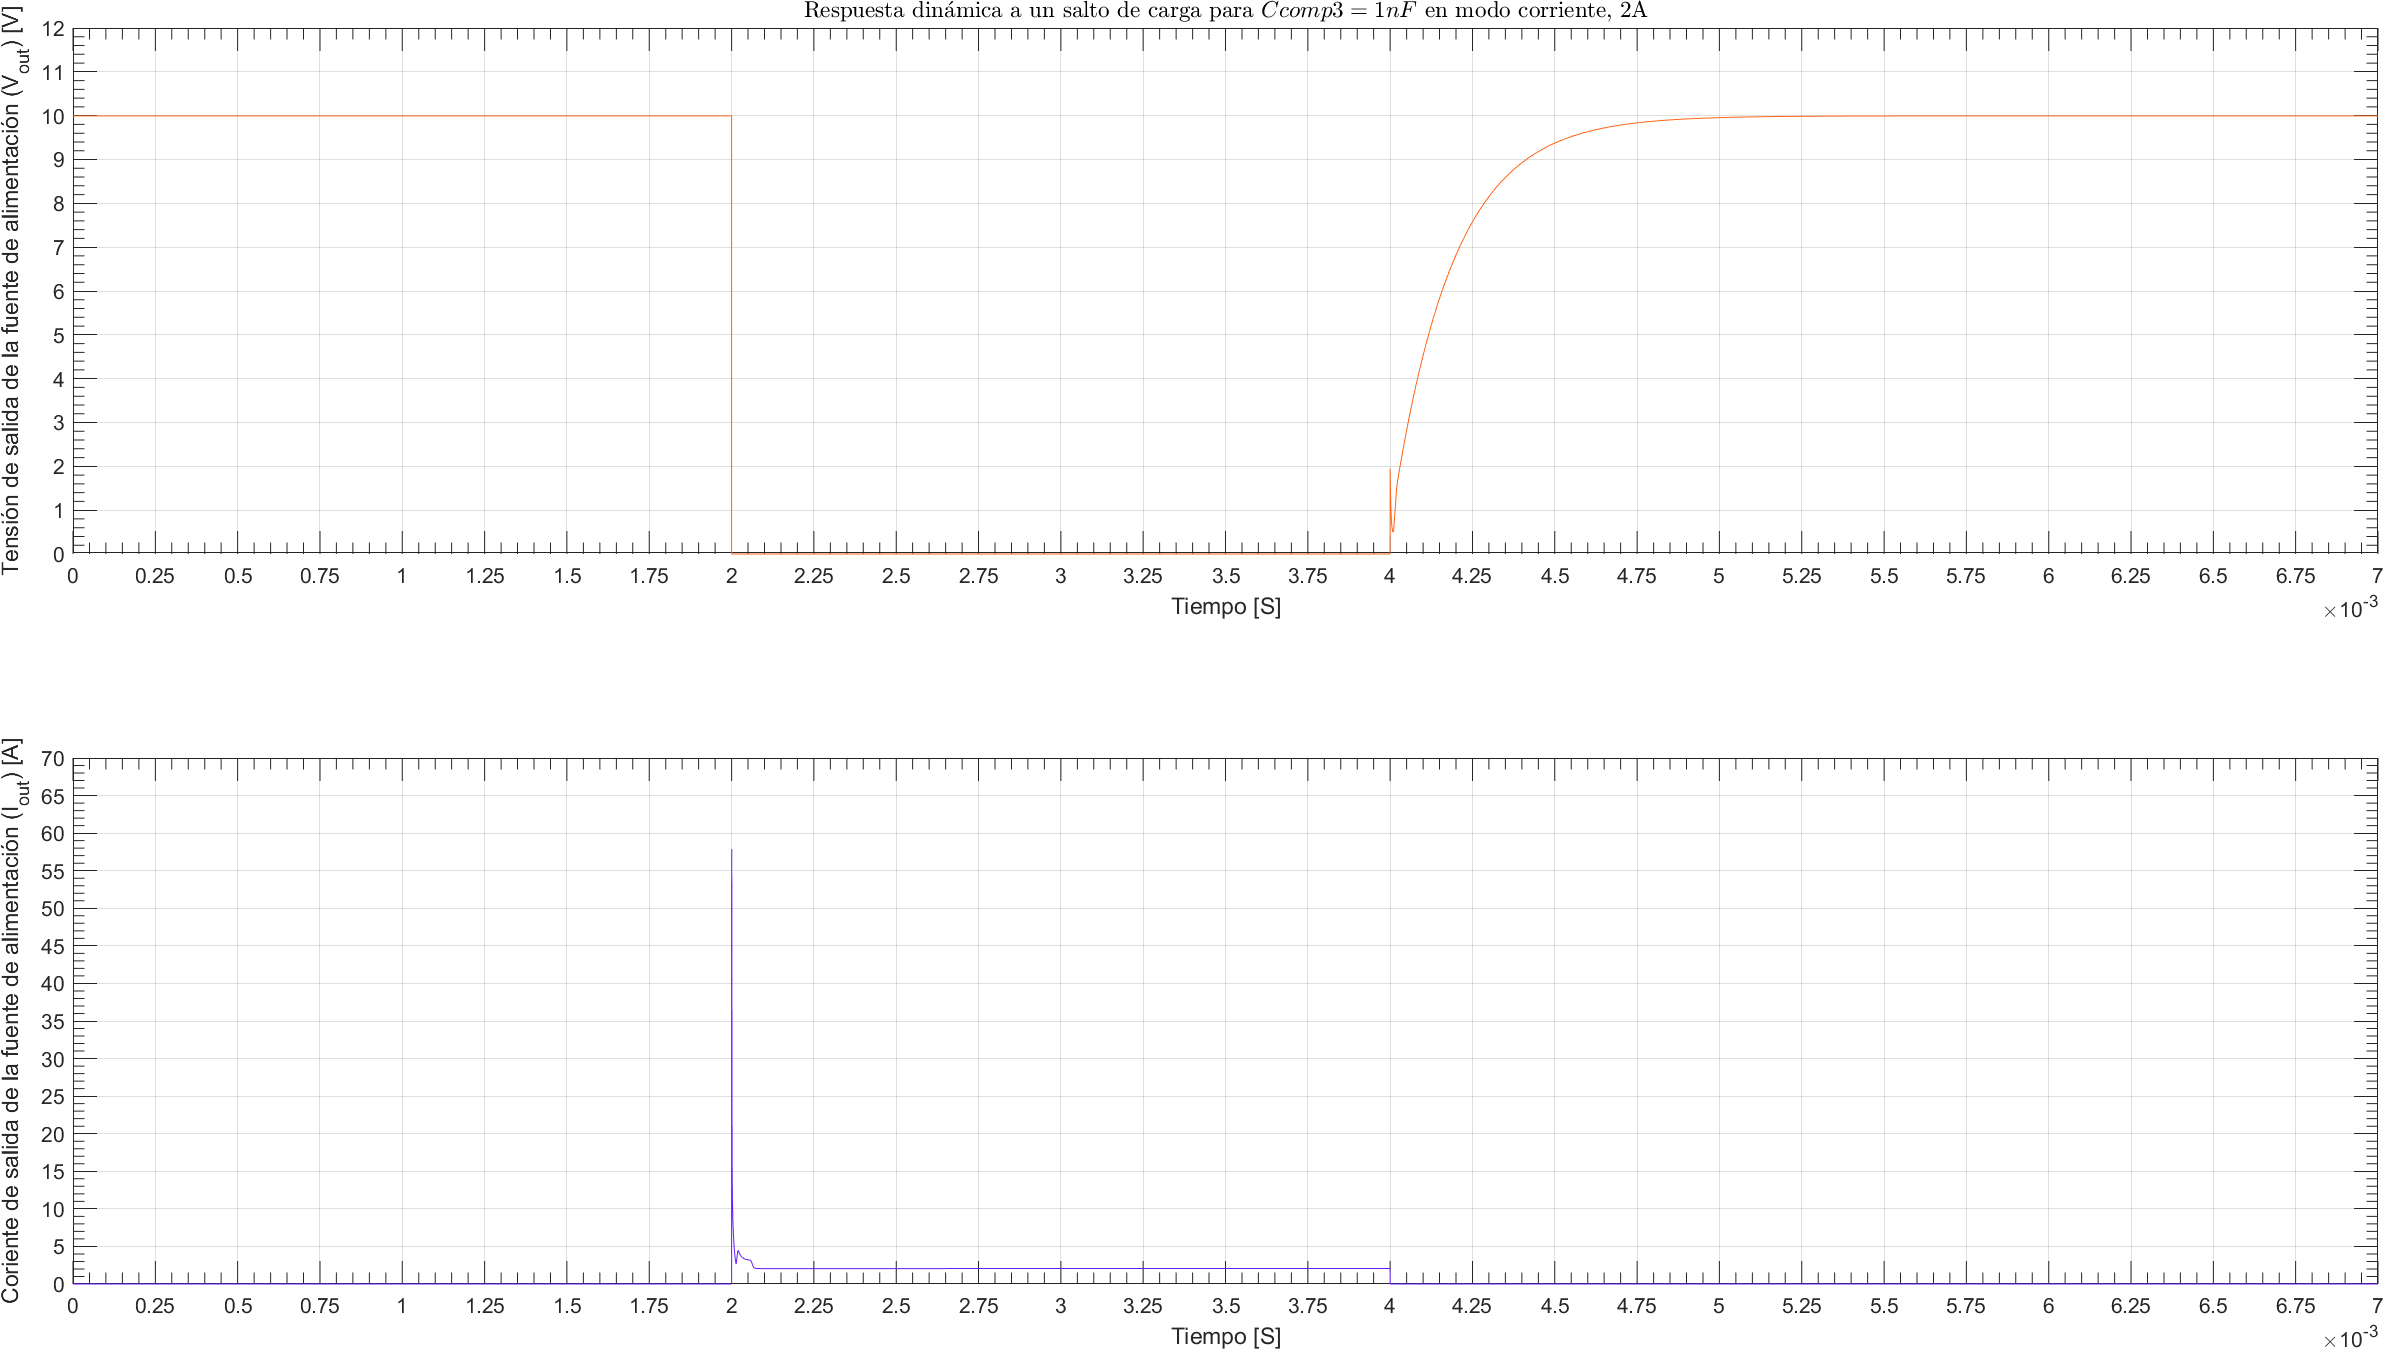
\includegraphics[width=1.1 \textwidth, angle=90]{./img/plots/dynamic/power_supply_CCOMP3_1n_STEP_Modo3.png}
\caption{\label{fig:fig_power_supply_CCOMP3_STEP_1n_Modo3}\footnotesize{Respuesta dinámica en modo corriente, $I_{out} = 2 \si[per-mode=symbol]{\ampere}$, para $C_{comp_{3}} = 1 \si[per-mode=symbol]{\nano\farad} $.}}
\end{center}
\end{figure}

\clearpage

\begin{figure}[H] %htb
\begin{center}
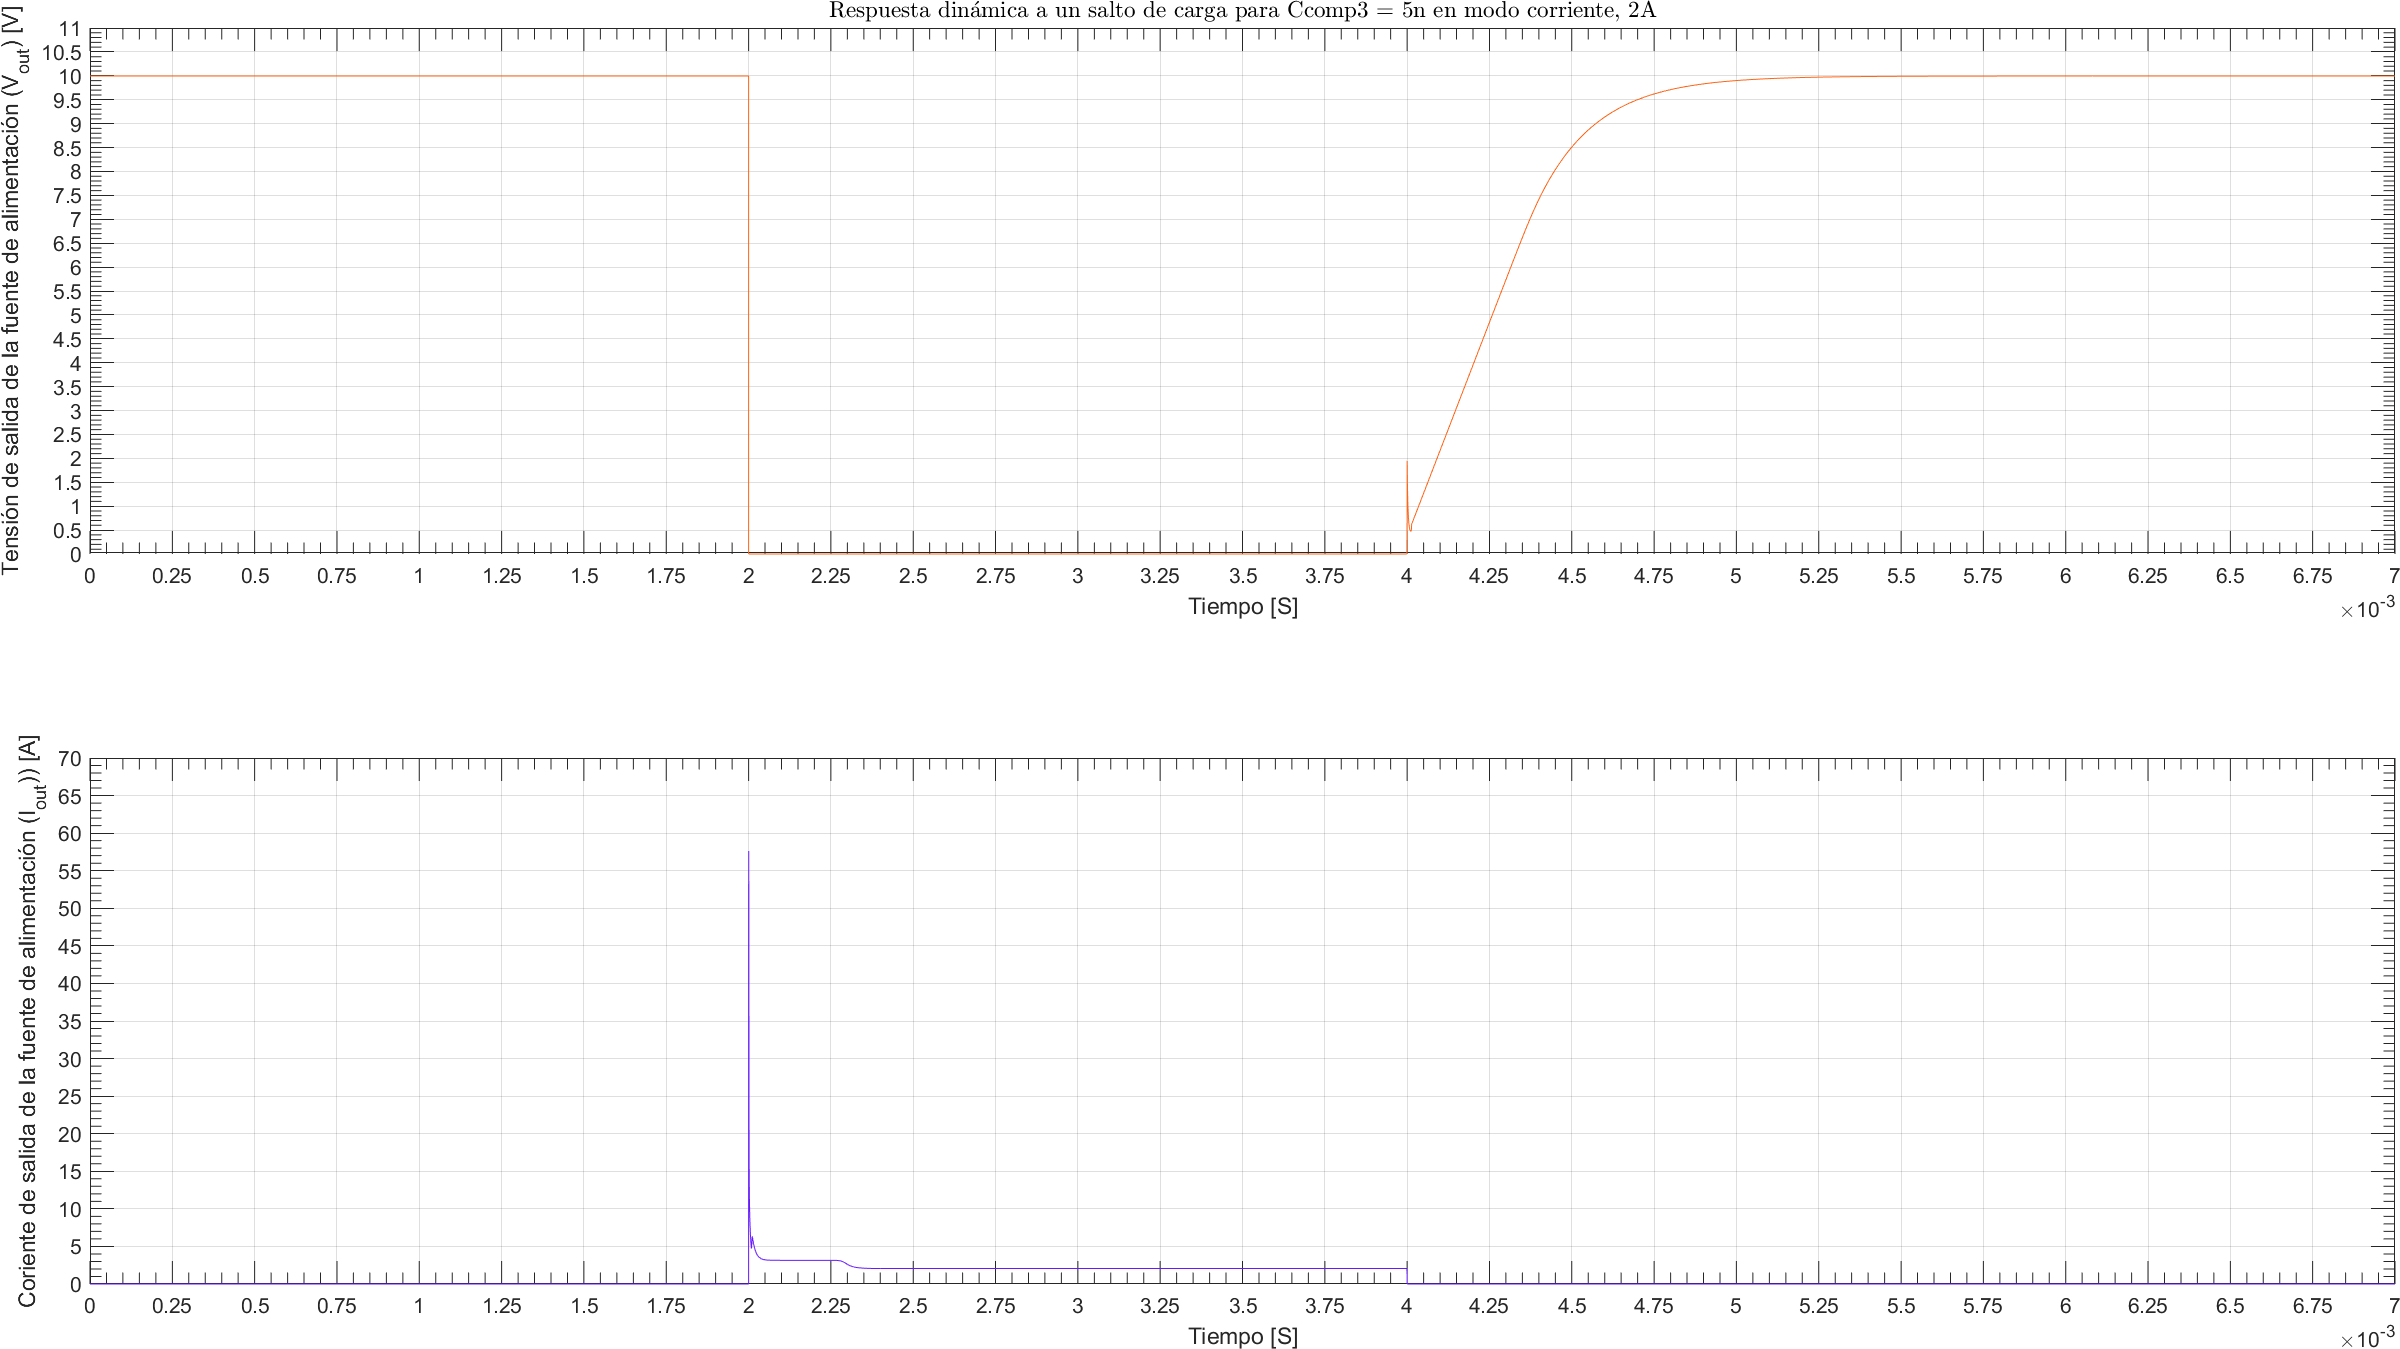
\includegraphics[width=1.1 \textwidth, angle=90]{./img/plots/dynamic/power_supply_CCOMP3_5n_STEP_Modo3.png}
\caption{\label{fig:fig_power_supply_CCOMP3_STEP_5n_Modo3}\footnotesize{Respuesta dinámica en modo corriente, $I_{out} = 2 \si[per-mode=symbol]{\ampere}$, para $C_{comp_{3}} = 5 \si[per-mode=symbol]{\nano\farad} $.}}
\end{center}
\end{figure}

\clearpage


\subsubsection{Análisis para $C_{comp_{3}}$ en modo corriente, $I_{out} = 200 \si[per-mode=symbol]{\milli\ampere}$, $R_{L} = 0 \si[per-mode=symbol]{\ohm}$}
% CCOMP3 MODO 4.

\clearpage

\begin{figure}[H] %htb
\begin{center}
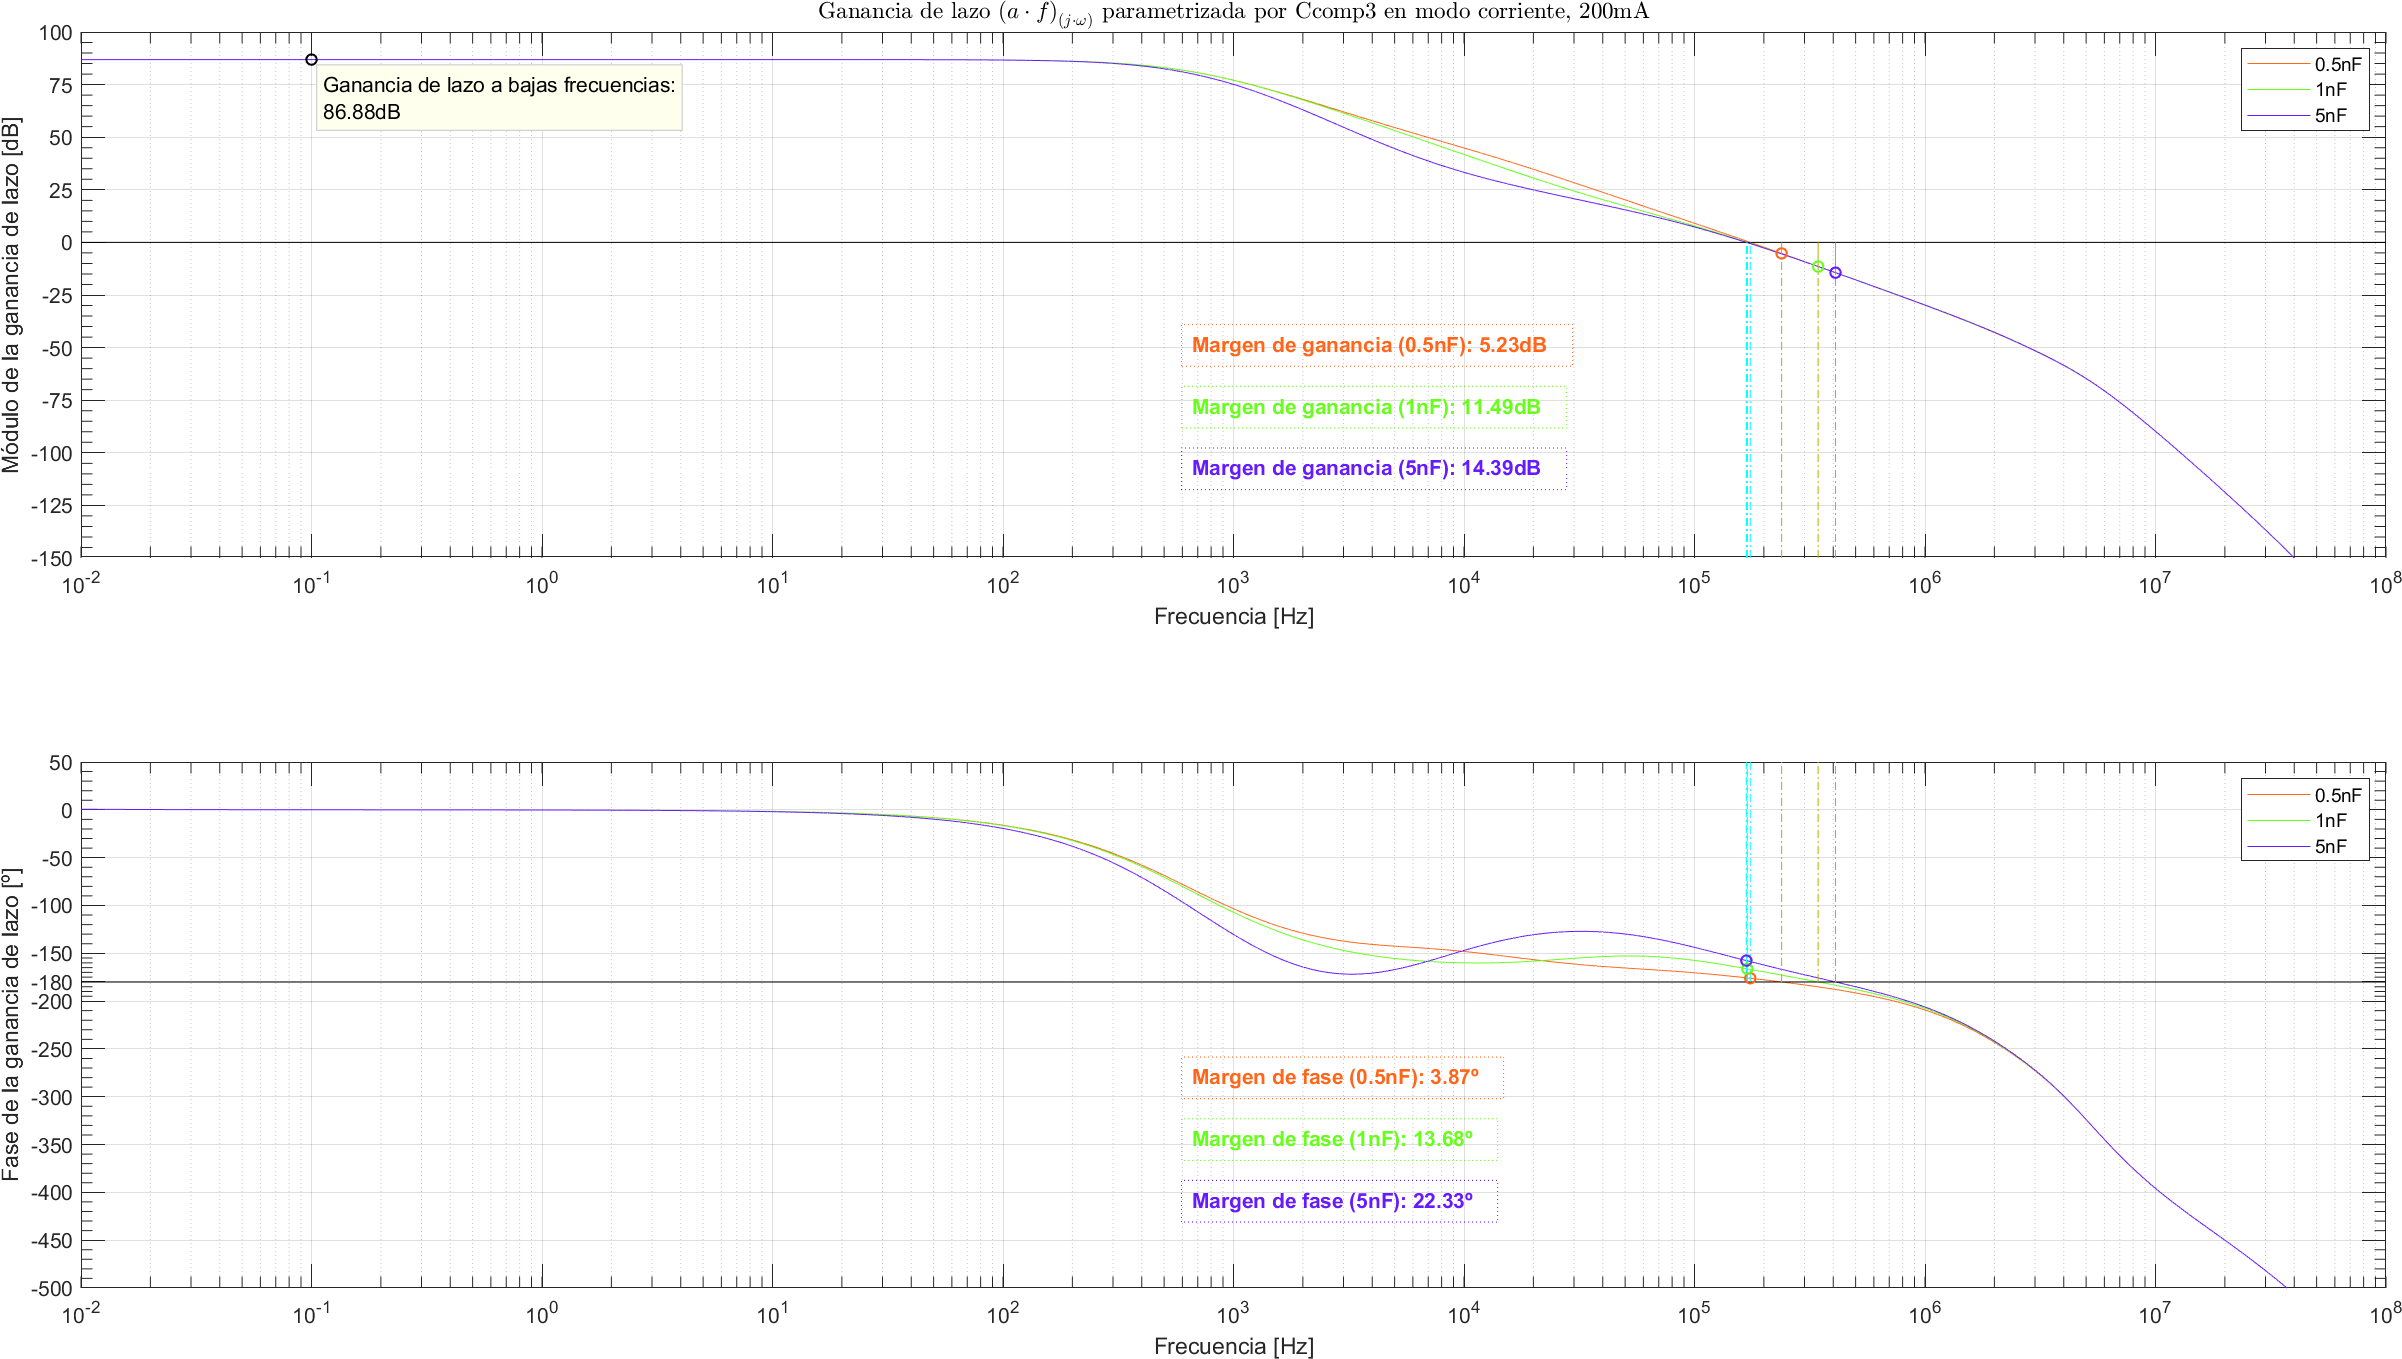
\includegraphics[width=1.1 \textwidth, angle=90]{./img/plots/loop/power_supply_CCOMP3_LOOP_Modo4.png}
\caption{\label{fig:fig_power_supply_CCOMP3_LOOP_Modo4}\footnotesize{Ganancia de lazo en modo corriente, $I_{out} = 200 \si[per-mode=symbol]{\milli\ampere}$, en función de la frecuencia parametrizada por $C_{comp_{3}}$.}}
\end{center}
\end{figure}


\clearpage

\begin{figure}[H] %htb
\begin{center}
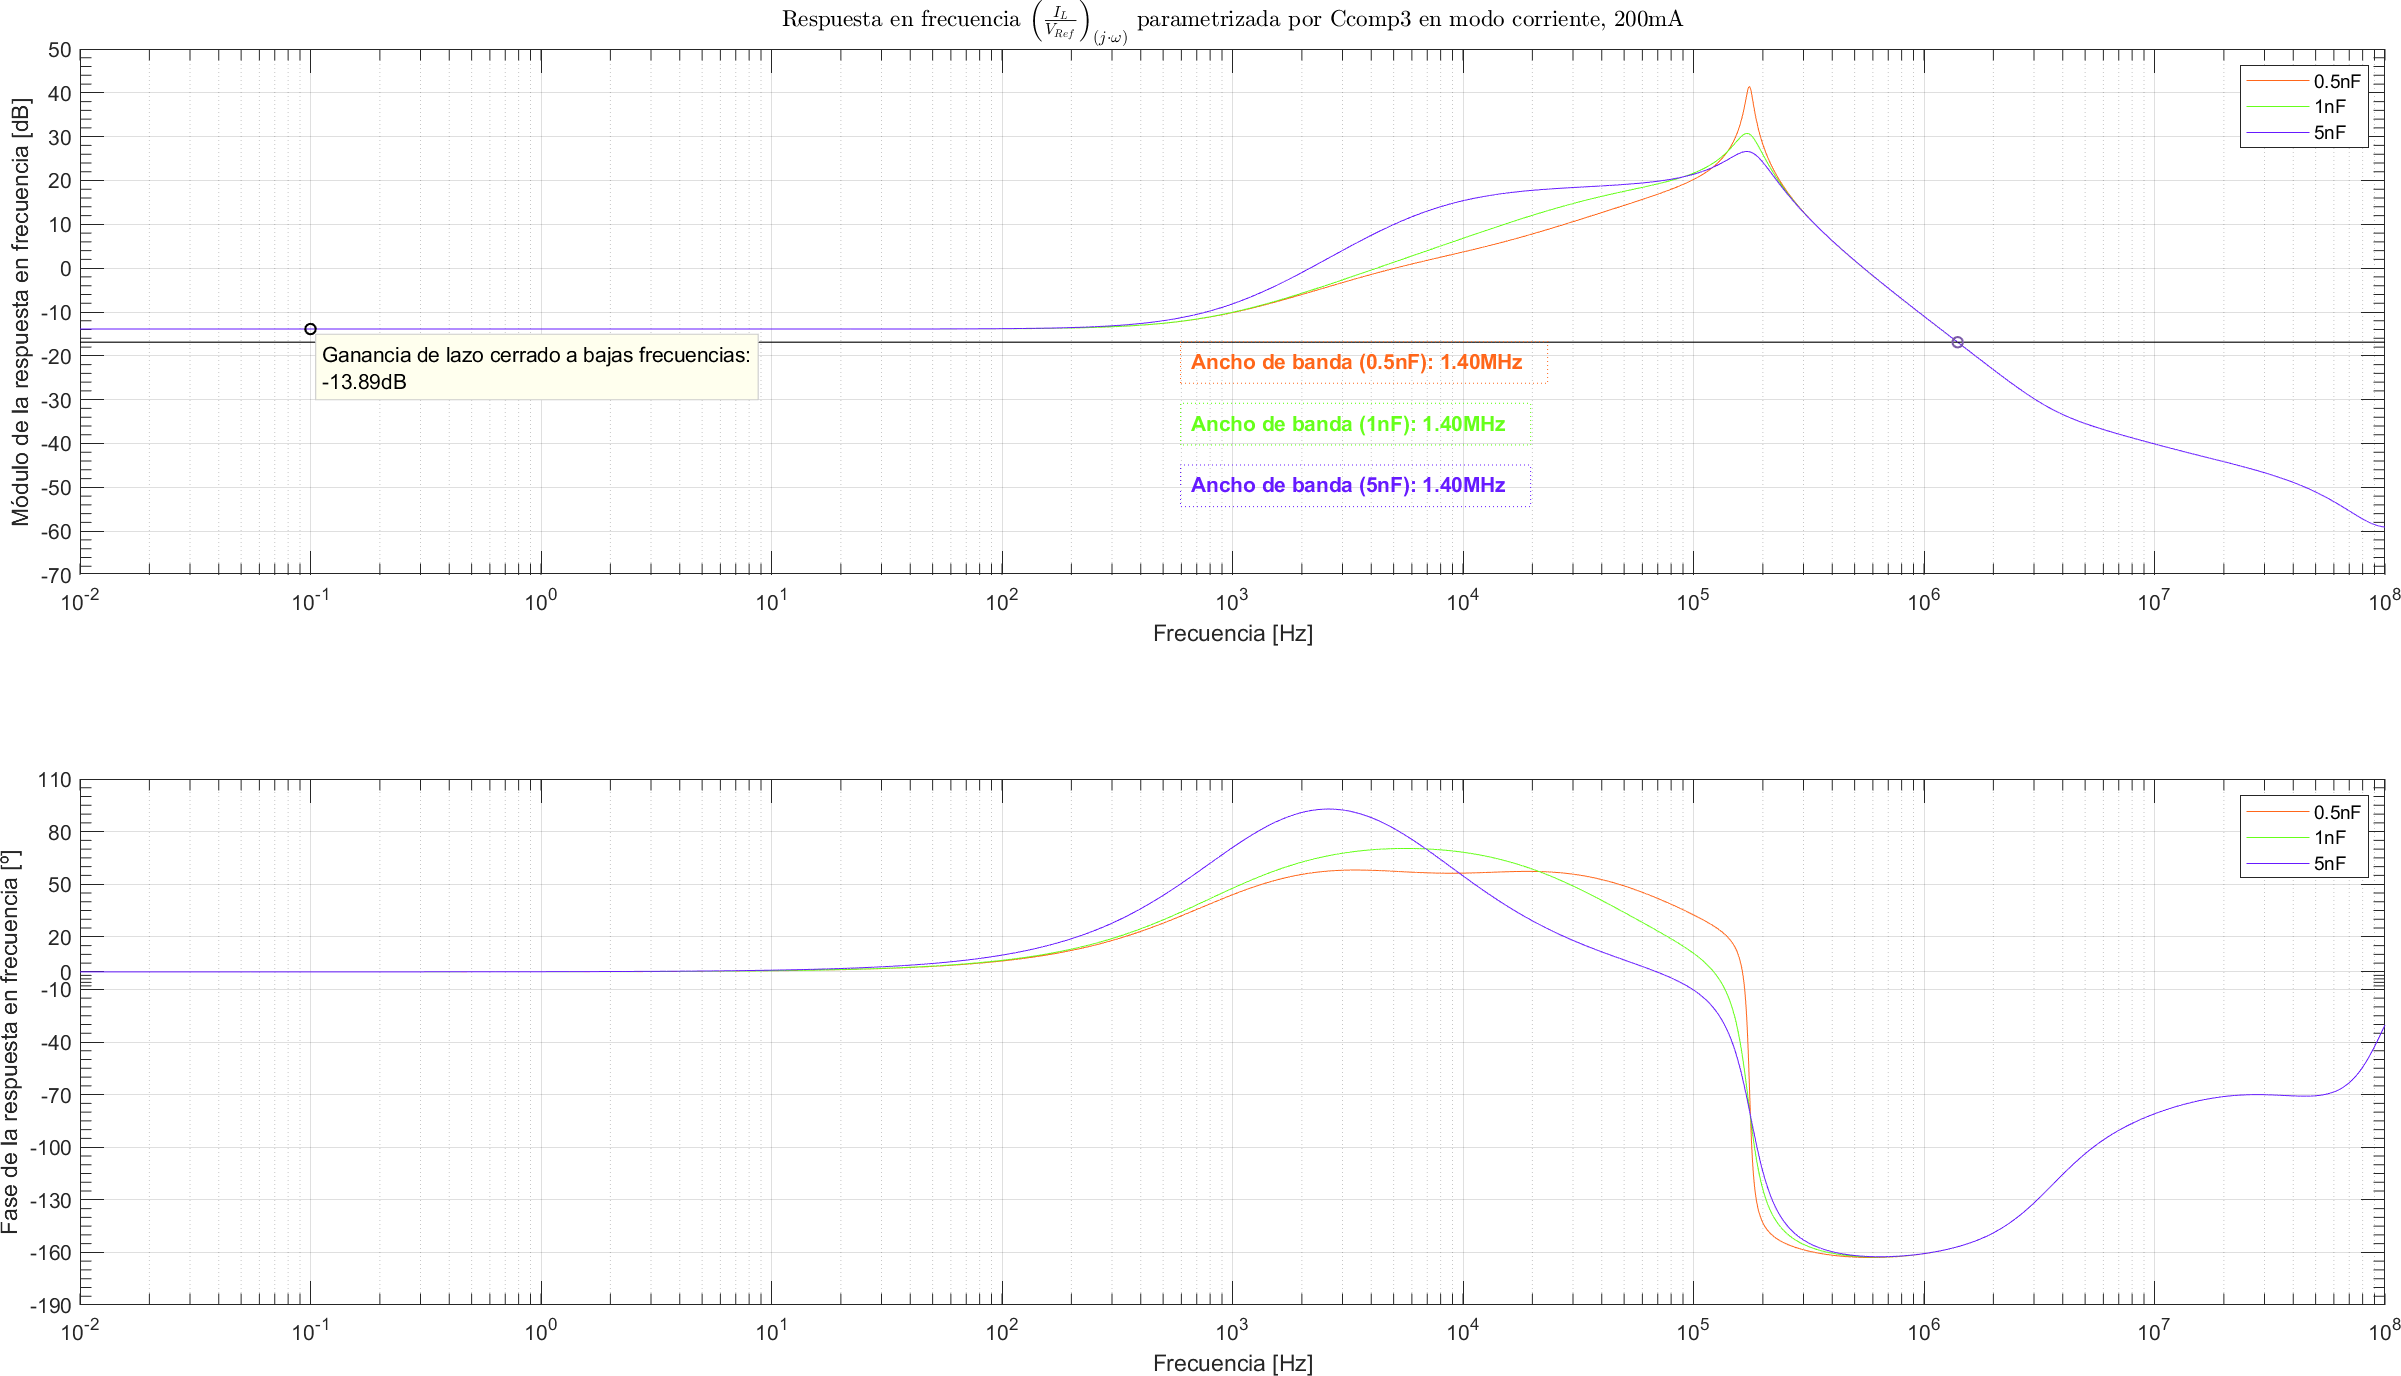
\includegraphics[width=1.1 \textwidth, angle=90]{./img/plots/rf/power_supply_CCOMP3_RF_Modo4.png}
\caption{\label{fig:fig_power_supply_CCOMP3_RF_Modo4}\footnotesize{Respuesta en frecuencia en modo corriente, $I_{out} = 200 \si[per-mode=symbol]{\milli\ampere}$, en función de la frecuencia parametrizada por $C_{comp_{3}}$.}}
\end{center}
\end{figure}

\clearpage

\begin{figure}[H] %htb
\begin{center}
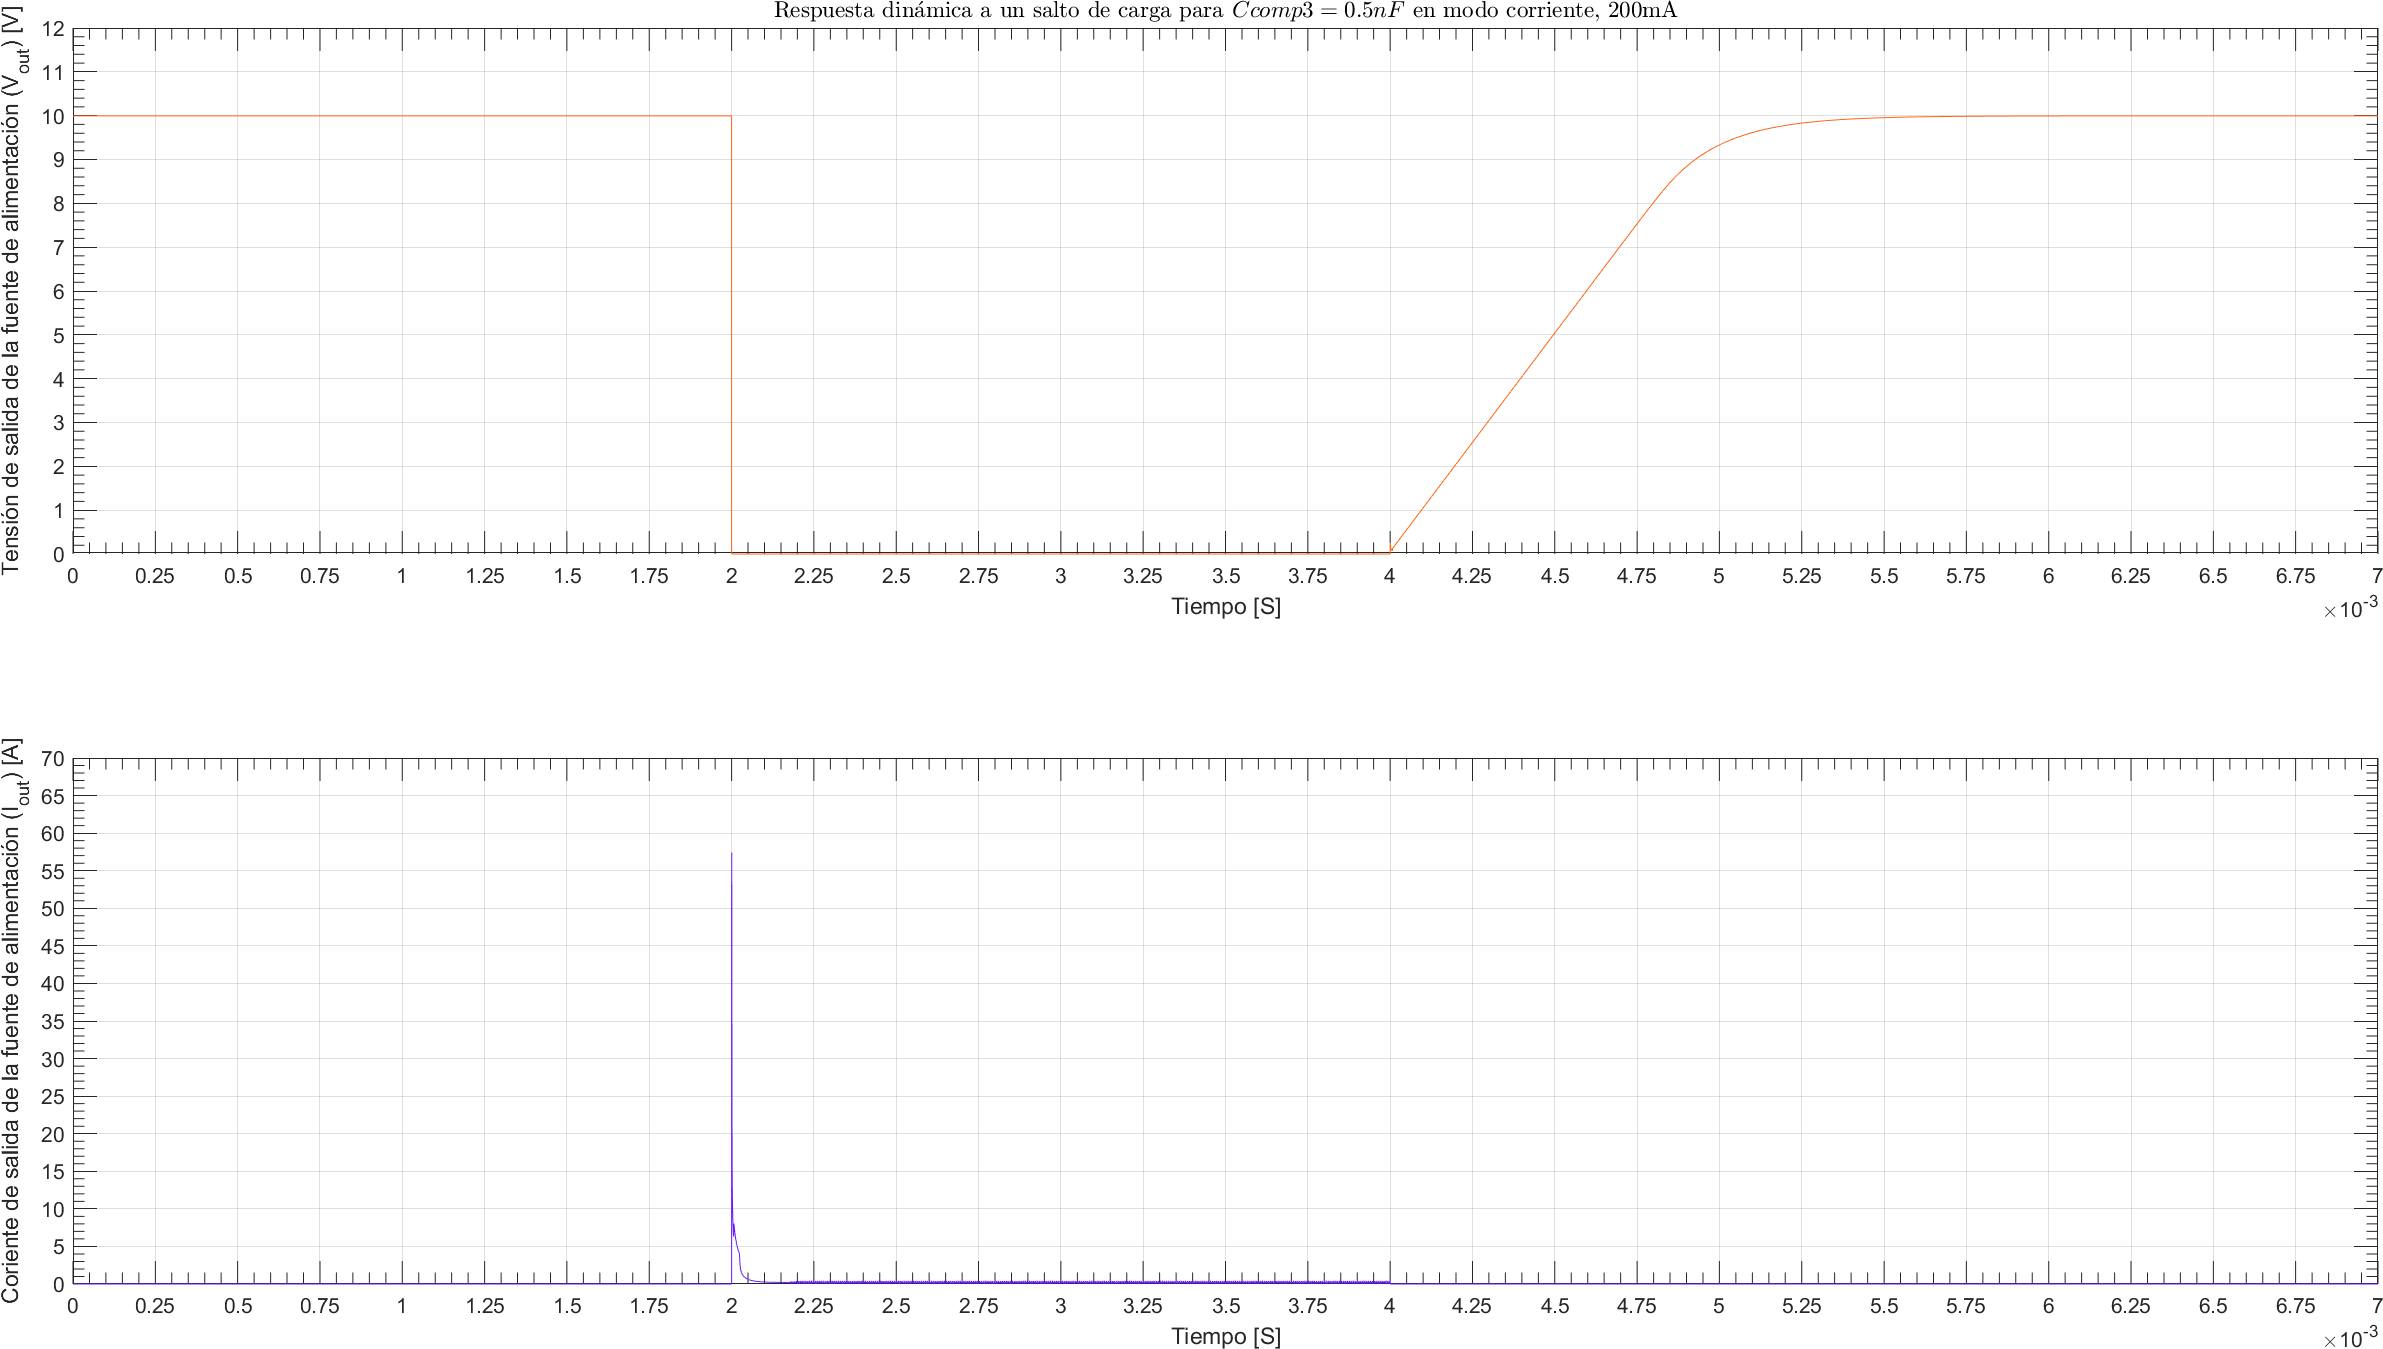
\includegraphics[width=1.1 \textwidth, angle=90]{./img/plots/dynamic/power_supply_CCOMP3_0_5n_STEP_Modo4.png}
\caption{\label{fig:fig_power_supply_CCOMP3_STEP_0_5n_Modo4}\footnotesize{Respuesta dinámica en modo corriente, $I_{out} = 200 \si[per-mode=symbol]{\milli\ampere}$, para $C_{comp_{3}} = 0.5 \si[per-mode=symbol]{\nano\farad} $.}}
\end{center}
\end{figure}

\clearpage

\begin{figure}[H] %htb
\begin{center}
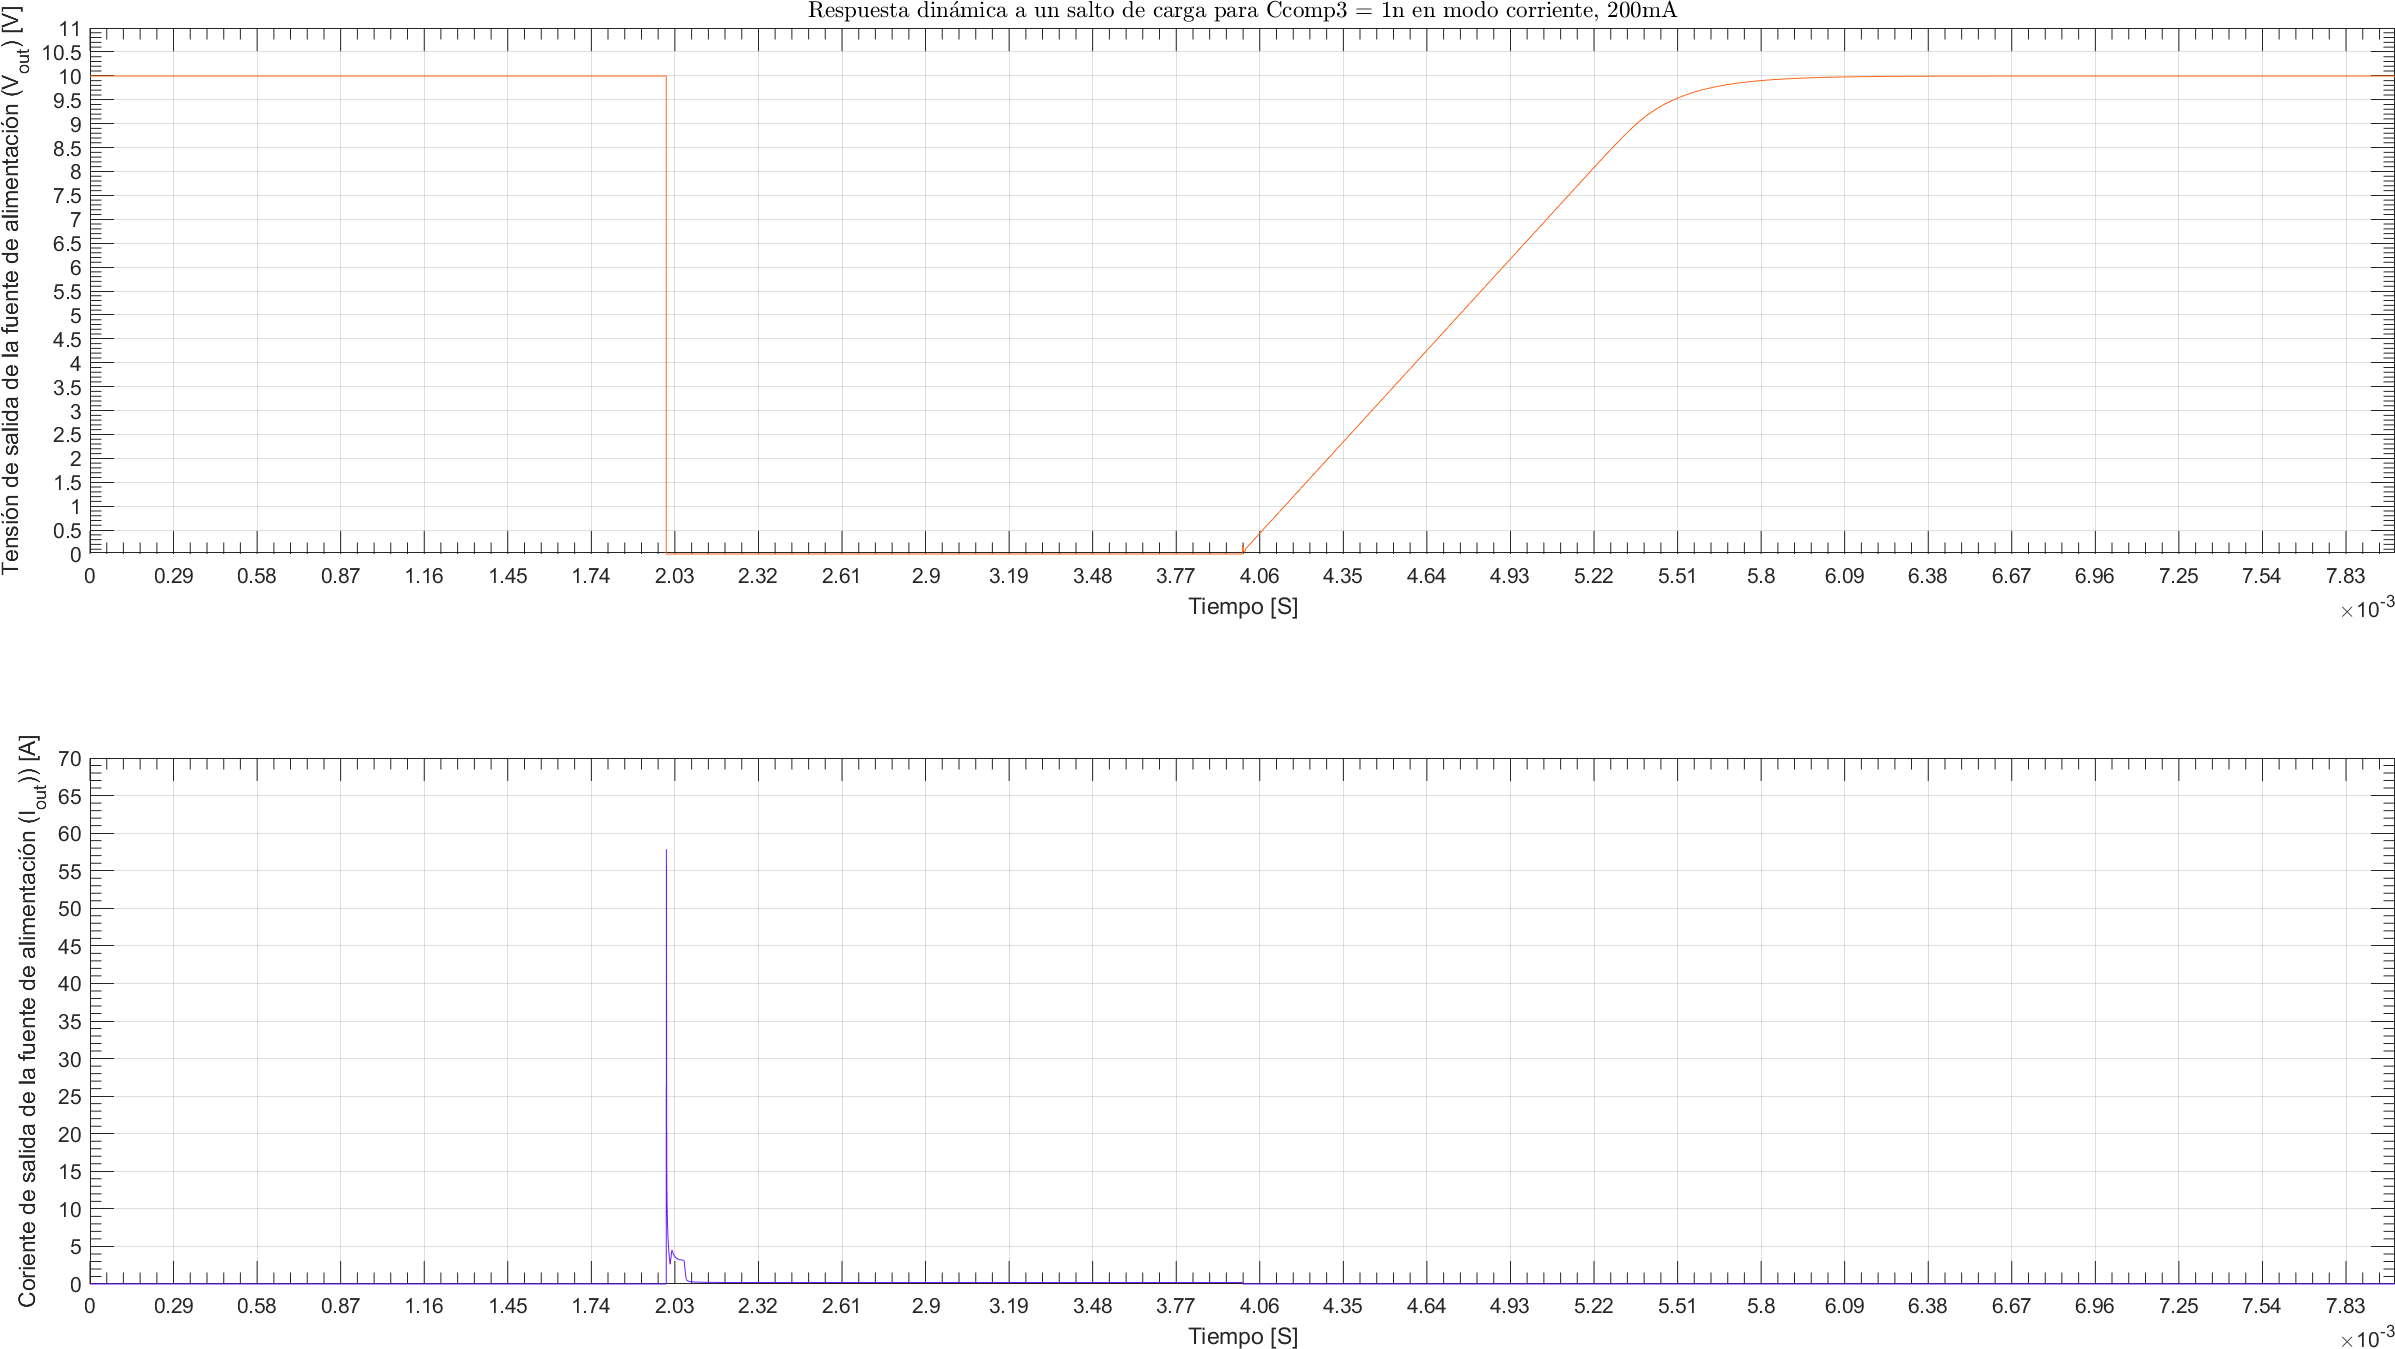
\includegraphics[width=1.1 \textwidth, angle=90]{./img/plots/dynamic/power_supply_CCOMP3_1n_STEP_Modo4.png}
\caption{\label{fig:fig_power_supply_CCOMP3_STEP_1n_Modo4}\footnotesize{Respuesta dinámica en modo corriente, $I_{out} = 200 \si[per-mode=symbol]{\milli\ampere}$, para $C_{comp_{3}} = 1 \si[per-mode=symbol]{\nano\farad} $.}}
\end{center}
\end{figure}

\clearpage

\begin{figure}[H] %htb
\begin{center}
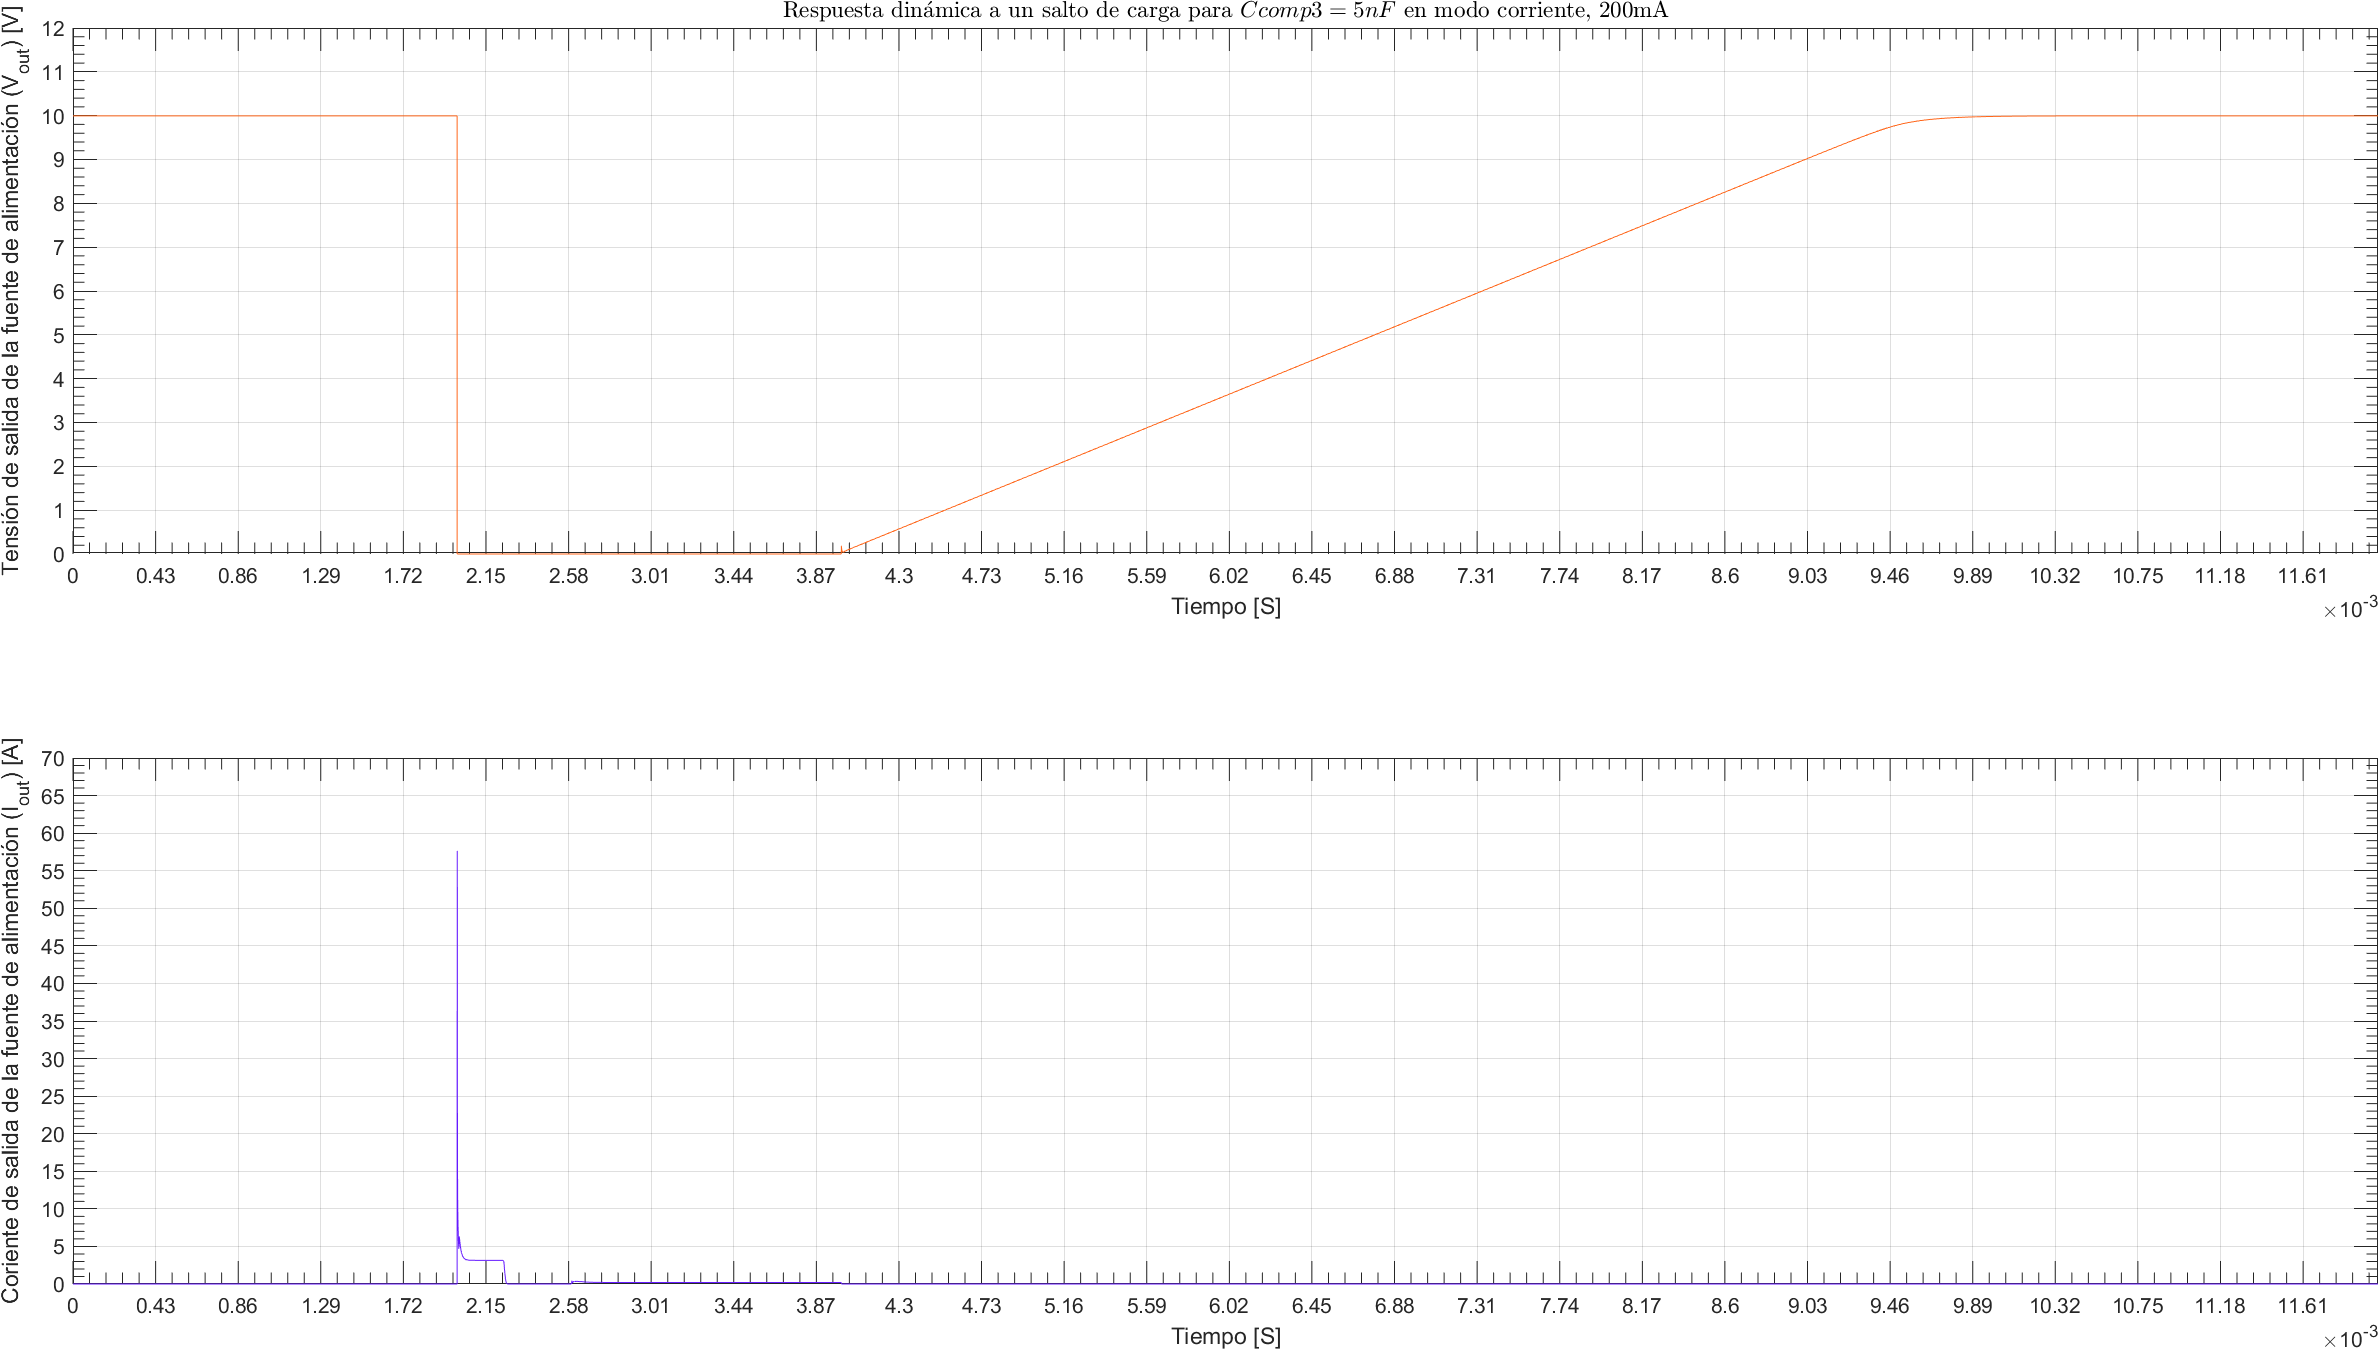
\includegraphics[width=1.1 \textwidth, angle=90]{./img/plots/dynamic/power_supply_CCOMP3_5n_STEP_Modo4.png}
\caption{\label{fig:fig_power_supply_CCOMP3_STEP_5n_Modo4}\footnotesize{Respuesta dinámica en modo corriente, $I_{out} = 200 \si[per-mode=symbol]{\milli\ampere}$, para $C_{comp_{3}} = 5 \si[per-mode=symbol]{\nano\farad} $.}}
\end{center}
\end{figure}

\clearpage




